\documentclass[12pt, spanish]{article}
\usepackage[spanish]{babel}
\selectlanguage{spanish}
\usepackage{natbib}
\usepackage{url}
\usepackage[utf8x]{inputenc}
\usepackage{graphicx}
\graphicspath{{images/}}
\usepackage{array}
\usepackage{float}
\usepackage{siunitx}
\usepackage[table,xcdraw,dvipsnames]{xcolor}
\usepackage{longtable}
\usepackage{parskip}
\usepackage{fancyhdr}
\usepackage{vmargin}
\usepackage{listings}
\usepackage{adjustbox}
\usepackage{subfig}
\usepackage{minted}
\usepackage[shortlabels]{enumitem}
\setlist[enumerate]{
labelsep=8pt,
labelindent=0.3\parindent,
itemindent=0pt,
leftmargin=*,
before=\setlength{\listparindent}{-\leftmargin},
}

\def\code#1{\texttt{#1}}
\usepackage[default]{sourcesanspro}
\usepackage{tcolorbox}
\usepackage{etoolbox}
\BeforeBeginEnvironment{minted}{\begin{tcolorbox}}%
\AfterEndEnvironment{minted}{\end{tcolorbox}}%

\setmarginsrb{2 cm}{1 cm}{2 cm}{2 cm}{1 cm}{1.5 cm}{1 cm}{1.5 cm}

\title{Práctica 1: Análisis de Eficiencia de Algoritmos \hspace{0.05cm} }
\date{}
\author{
Yunkai Lin Pan: 20\% \\
Alfonso Jesús Piñera Herrera: 20\% \\
Álvaro Hernández Coronel: 20\%  \\
Jaime Castillo Uclés: 20\% \\
Yeray López Ramírez: 20\% \\
}

\renewcommand*\contentsname{hola}

\makeatletter
\let\thetitle\@title
\let\theauthor\@author
\let\thedate\@date
\makeatother

\pagestyle{fancy}
\fancyhf{}
\rhead{}
\chead{\thedate}
\lhead{\thetitle}
\cfoot{\thepage}

\begin{document}
%%%%%%%%%%%%%%%%%%%%%%%%%%%%%%%%%%%%%%%%%%%%%%%%%%%%%%%%%%%%%%%%%%%%%%%%%%%%%%%%%%%%%%%%%
\begin{titlepage}
  \centering
  \vspace*{0.5 cm}
  
\includegraphics[scale = 0.50]{ugr.png}\\[1.0 cm]
  %\textsc{\LARGE Universidad de Granada}\\[2.0 cm]   
  \textsc{\huge Grado en Ingeniería Informática}\\[0.5 cm]
  \rule{\linewidth}{0.2 mm} \\[0.4 cm]
  { \huge \bfseries \thetitle}\\
  \rule{\linewidth}{0.2 mm} \\[1.5 cm]
  
  \begin{minipage}{0.4\textwidth}
    \begin{flushleft} \large
        \emph{Autores:}\\

        \small \theauthor
        \end{flushleft}
        \end{minipage}~
        \begin{minipage}{0.4\textwidth}
        \begin{flushright} \large
        \emph{Curso:2ºC \\
        Asignatura: Algorítmica \\
        Fecha: 22 de Marzo de 2022 \\
        Grupo de prácticas: C2 \\
        Número de grupo: 3}
    \end{flushright}
\end{minipage}\\[1 cm]


\vfill
  
\end{titlepage}

\newpage

%%%%%%%%%%%%%%%%%%%%%%%%%%%%%%%%%%%%%%%%%%%%%%%%%%%%%%%%%%%%%%%%%%%%%%%%%%%%%%%%%%%%%%%%%


\tableofcontents
\pagebreak

%%%%%%%%%%%%%%%%%%%%%%%%%%%%%%%%%%%%%%%%%%%%%%%%%%%%%%%%%%%%%%%%%%%%%%%%%%%%%%%%%%%%%%%%%

\section{Descripción del problema}
En esta práctica analizaremos de forma \textbf{empírica} e \textbf{híbrida} distintos algorítmos.

\section{Algoritmos de Ordenación}
En esta parte trataremos cuatro de los algoritmos de ordenación más conocidos. Los dividiremos en \emph{cuadráticos} y \emph{logarítmicos}:

\subsection{Eficiencia n²}
Los algoritmos a calcular su eficiencia empírica que tienen este tipo de eficiencia son el algoritmo de la \textbf{burbuja} y de la \textbf{inserción}.
Empezamos con el algoritmo de la \emph{burbuja}.

\subsubsection{Ordenación por Burbuja}
La función proporcionada para este algoritmo es la siguiente:
\begin{minted}{c++}
 inline void burbuja(int T[], int num_elem)
{
 burbuja_lims(T, 0, num_elem);
}

static void burbuja_lims(int T[], int inicial, int final)
{
 int i, j;
 int aux;
 for (i = inicial; i < final - 1; i++)
   for (j = final - 1; j > i; j--)
     if (T[j] < T[j-1])
 {
   aux = T[j];
   T[j] = T[j-1];
   T[j-1] = aux;
 }
}
\end{minted}

\renewcommand{\arraystretch}{1.25}
\newpage
Al ejecutar \textcolor{BrickRed}{\code{./burbuja}} con los valores predeterminados del compilador:
\begin{longtable}{|c|c|}
\hline
\textbf{Tamaño} & \textbf{Tiempo(seg)} \\ \hline
5000   & 0.0858651   \\ \hline
10000  & 0.247879    \\ \hline
15000  & 0.585624    \\ \hline
20000  & 1.05817     \\ \hline
25000  & 1.67296     \\ \hline
30000  & 2.45572     \\ \hline
35000  & 3.37203     \\ \hline
40000  & 4.44497     \\ \hline
45000  & 5.69015     \\ \hline
50000  & 7.0206      \\ \hline
55000  & 8.62408     \\ \hline
60000  & 10.2721     \\ \hline
65000  & 12.0943     \\ \hline
70000  & 14.0043     \\ \hline
75000  & 16.1324     \\ \hline
80000  & 18.3781     \\ \hline
85000  & 20.7872     \\ \hline
90000  & 23.3628     \\ \hline
95000  & 26.6501     \\ \hline
100000 & 30.6623     \\ \hline
105000 & 34.4759     \\ \hline
110000 & 35.5128     \\ \hline
115000 & 43.256      \\ \hline
120000 & 44.2151     \\ \hline
125000 & 46.153      \\ \hline
\end{longtable}


\newpage

Al usar gnuplot para graficar los datos anteriores, se crea la siguiente gráfica:
\begin{figure}[H]
  \centering
  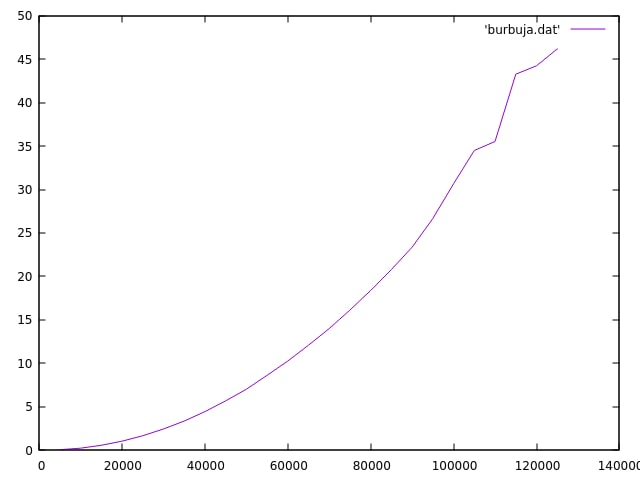
\includegraphics[scale = 0.8]{burbuja.png}
\end{figure}

La eficiencia híbrida calculada mediante gnuplot da como resultado el siguiente fichero  \textbf{\textcolor{ForestGreen}{\code{fit.log}}}:

\begin{minted}{text}
FIT:    data read from 'burbuja.dat'
       #datapoints = 25
function used for fitting: f(x)
       f(x) = a0*x*x+a1*x+a2
iter      chisq       delta/lim  lambda   a0            a1            a2
  0 1.3460545235e+21   0.00e+00  4.24e+09    1.000000e+00   1.000000e+00
 13 1.6690141492e+01  -1.14e-05  4.24e-04    3.336682e-09  -3.675681e-05
After 13 iterations the fit converged.
Final set of parameters            Asymptotic Standard Error
=======================            ==========================
a0              = 3.33668e-09      +/- 1.502e-10    (4.501%)
a1              = -3.67568e-05     +/- 2.011e-05    (54.72%)
a2              = 0.402602         +/- 0.5674       (140.9%)
correlation matrix of the fit parameters:
                a0     a1     a2
a0              1.000
a1             -0.971  1.000
a2              0.774 -0.884  1.000
\end{minted}

De aquí concluimos que la formula ajustada es:

\[f(x)=\num{3.33668e-09}x² - \num{3.67568e-05}x + 0.402602\]

Tras representar la función ajustada anterior en la gráfica de puntos podemos ver que se ajustan perfectamente:
\begin{figure}[H]
  \centering
  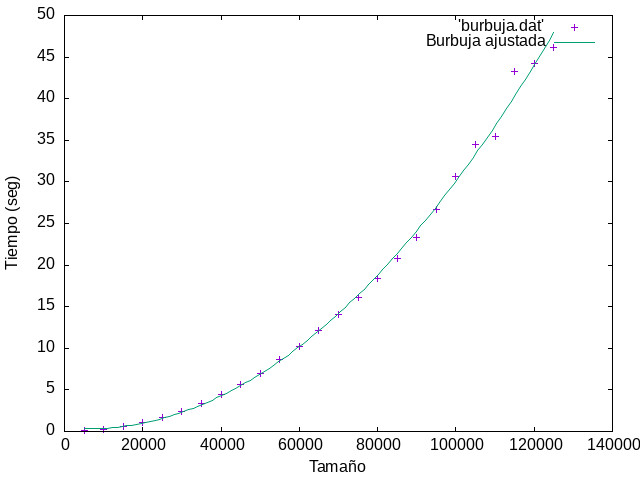
\includegraphics[scale = 0.8]{burbujaAjustada.png}
\end{figure}

\subsubsection{Ordenación por Inserción}
La función del algoritmo de inserción analizado es la siguiente:

\begin{minted}{c++}
static void insercion_lims(int T[], int inicial, int final){
  int i, j, aux;
  for (i = inicial + 1; i < final; i++) {
	j = i;
	while ((T[j] < T[j-1]) && (j > 0)) {
  	aux = T[j];
  	T[j] = T[j-1];
  	T[j-1] = aux;
  	j--;
	}
  }
}
\end{minted}

\newpage

La tabla de datos resultante en el PC de nuestro compañero Álvaro es:
\begin{longtable}{|c|c|}
\hline
\textbf{Tamaño} & \textbf{Tiempo(seg)} \\ \hline
5000   & 0.0398803   \\ \hline
10000  & 0.107249    \\ \hline
15000  & 0.245123    \\ \hline
20000  & 0.419207    \\ \hline
25000  & 0.630739    \\ \hline
30000  & 0.911298    \\ \hline
35000  & 1.27238     \\ \hline
40000  & 1.60618     \\ \hline
45000  & 2.05534     \\ \hline
50000  & 2.51724     \\ \hline
55000  & 3.06278     \\ \hline
60000  & 3.63798     \\ \hline
65000  & 4.22758     \\ \hline
70000  & 9.06372     \\ \hline
75000  & 9.3657      \\ \hline
80000  & 10.3132     \\ \hline
85000  & 7.27995     \\ \hline
90000  & 8.11229     \\ \hline
95000  & 9.09415     \\ \hline
100000 & 10.0099     \\ \hline
105000 & 11.0659     \\ \hline
110000 & 14.0415     \\ \hline
115000 & 13.2668     \\ \hline
120000 & 14.474      \\ \hline
125000 & 15.6717     \\ \hline
\end{longtable}

\begin{center}
Como podemos entrever, hay algunos picos inesperados para ciertos tamaños.

\newpage

Al graficar la tabla de datos, efectivamente vemos los picos más claramente:
\end{center}

\begin{figure}[H]
  \centering
  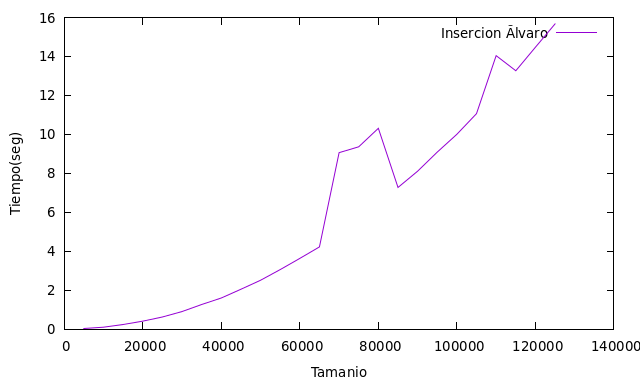
\includegraphics[scale = 0.7]{insercionAlvaro.png}
  \caption{Algoritmo de Inserción en el PC de Álvaro}
\end{figure}

Desconocemos el porqué de este resultado errático, también sucede en el ordenador personal del compañero Yeray:

\begin{figure}[H]
  \centering
  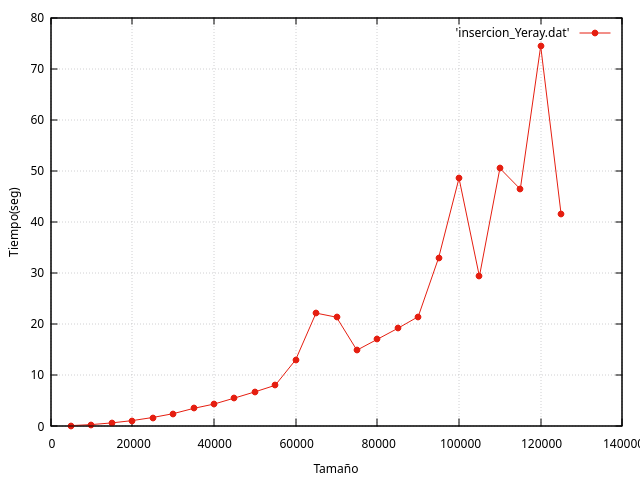
\includegraphics[scale = 0.7]{insercionYeray.png}
\end{figure}


Al intentar ajustar los datos de antes vemos que el porcentaje de error es inusualmente alto:
\begin{minted}{text}
 **********************************************************************
Mon Mar 21 16:02:10 2022


FIT:	data read from "insercion.dat"
    	format = z
    	#datapoints = 25
    	residuals are weighted equally (unit weight)

function used for fitting: f(x)
    f(x) = a0*x*x+a1*x+a2
fitted parameters initialized with current variable values

iter  	chisq   delta/lim  lambda   a0        	a1
   0 1.3460545288e+21   0.00e+00  4.24e+09	1.000000e+00
  13 3.6180941721e+01  -5.50e-05  4.24e-04	6.294092e-10

After 13 iterations the fit converged.
final sum of squares of residuals : 36.1809
rel. change during last iteration : -5.50109e-10

degrees of freedom	(FIT_NDF)                    	: 22
rms of residuals  	(FIT_STDFIT) = sqrt(WSSR/ndf)	: 1.28242
variance of residuals (reduced chisquare) = WSSR/ndf   : 1.64459

Final set of parameters        	Asymptotic Standard Error
=======================        	==========================
a0          	= 6.29409e-10  	+/- 2.211e-10	(35.13%)
a1          	= 5.46974e-05  	+/- 2.961e-05	(54.14%)
a2          	= -0.933148    	+/- 0.8354   	(89.52%)

correlation matrix of the fit parameters:
                a0     a1     a2
a0              1.000
a1             -0.971  1.000
a2              0.774 -0.884  1.000
\end{minted}

La función ajustada que nos genera es:

\[f(x)=\num{6.29409e-10}x² + \num{5.46974e-05}x - 0.933148\]

\newpage

Al ajustarla vemos que la función pasa por el medio de los puntos:
\begin{figure}[H]
  \centering
  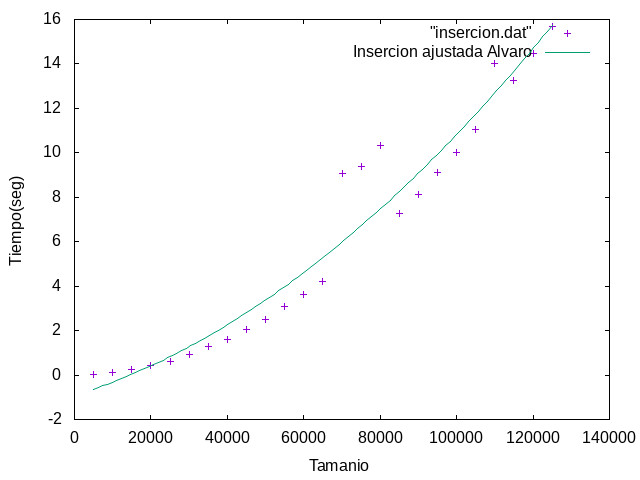
\includegraphics[scale = 0.8]{AjusteAlvaro.png}
  \caption{Ajuste en el PC de Álvaro}
\end{figure}


Sin embargo, tras ejecutar exactamente el mismo fichero fuente del algoritmo en el ordenador de Jaime obtenemos una tabla sin sorpresas:
\begin{longtable}{|c|c|}
\hline
\textbf{Tamaño} & \textbf{Tiempo(seg)} \\ \hline
5000   & 0.0286526   \\ \hline
10000  & 0.107456    \\ \hline
15000  & 0.208767    \\ \hline
20000  & 0.351672    \\ \hline
25000  & 0.552823    \\ \hline
30000  & 0.772061    \\ \hline
35000  & 1.08757     \\ \hline
40000  & 1.41086     \\ \hline
45000  & 1.62846     \\ \hline
50000  & 1.95397     \\ \hline
55000  & 2.31595     \\ \hline
60000  & 2.75238     \\ \hline
65000  & 3.25217     \\ \hline
70000  & 3.82004     \\ \hline
75000  & 4.35694     \\ \hline
80000  & 4.95242     \\ \hline
85000  & 5.61813     \\ \hline
90000  & 6.40346     \\ \hline
95000  & 7.37948     \\ \hline
100000 & 7.86567     \\ \hline
105000 & 8.78106     \\ \hline
110000 & 9.40774     \\ \hline
115000 & 10.3115     \\ \hline
120000 & 12.5462     \\ \hline
125000 & 12.1462     \\ \hline
\end{longtable}


Efectivamente al graficarla ésta se ajusta a una función cuadrática convencional a excepción de la última ejecución que sufre una bajada de medio segundo respecto a la anterior ejecución:
\begin{figure}[H]
  \centering
  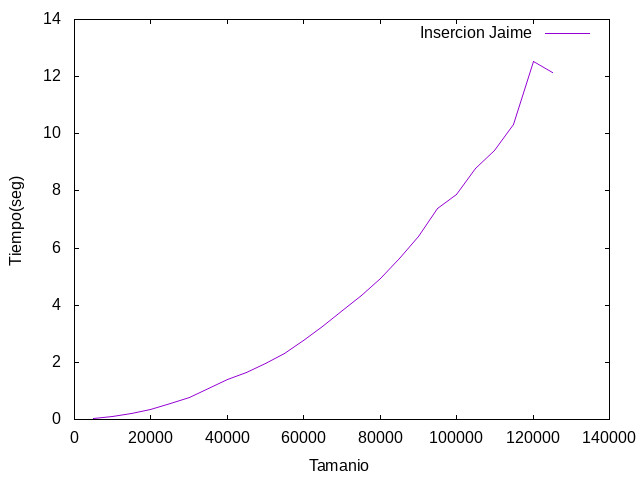
\includegraphics[scale = 0.8]{insercionJaime.png}
  \caption{Algoritmo de Inserción en el PC de Jaime}
\end{figure}

El ajuste queda finalmente:

\begin{minted}{text}
************************************************************************
Mon Mar 21 16:14:53 2022


FIT:	data read from "insercion2.dat"
    	format = z
    	#datapoints = 25
    	residuals are weighted equally (unit weight)

function used for fitting: f(x)
    f(x) = a0*x*x+a1*x+a2
fitted parameters initialized with current variable values

iter  	chisq          delta/lim  lambda    a0
   0 1.1054819544e+02   0.00e+00  3.59e+00	6.294092e-10
   4 1.4550871377e+00  -1.09e-03  3.59e-04	8.460509e-10

After 4 iterations the fit converged.
final sum of squares of residuals : 1.45509
rel. change during last iteration : -1.08883e-08

degrees of freedom	(FIT_NDF)                    	: 22
rms of residuals  	(FIT_STDFIT) = sqrt(WSSR/ndf)	: 0.257178
variance of residuals (reduced chisquare) = WSSR/ndf   : 0.0661403

Final set of parameters        	Asymptotic Standard Error
=======================        	==========================
a0          	= 8.46051e-10  	+/- 4.434e-11	(5.241%)
a1          	= -6.43769e-06 	+/- 5.938e-06	(92.24%)
a2          	= 0.144484     	+/- 0.1675   	(116%)

correlation matrix of the fit parameters:
            	a0   a1 	a2
a0          	1.000
a1         	-0.971  1.000
a2          	0.774 -0.884  1.000
\end{minted}

La función resultante del ajuste es similar a la anterior:

\[f(x) = \num{8.46051e-10}x² - \num{6.43769e-06}x + 0.144484\]

\newpage

Sin embargo, esta vez si pasa por los puntos de forma correcta:
\begin{figure}[H]
  \centering
  \includegraphics[scale = 1]{AjusteJaime.png}
  \caption{Ajuste del algoritmo de Inserción en el PC de Jaime}
\end{figure}


\subsection{Eficiencia n log(n)}
Los algoritmos de orden $n\;log(n)$ son el algoritmo de \textbf{mergesort} y el \textbf{quicksort} que son algoritmos de ordenación de vectores. Los explicamos a continuación:

\subsubsection{Ordenación por Mergesort}
Es uno de los algoritmos más eficientes de la práctica junto al Quicksort. Como veremos después, el set de datos no pasa del segundo.

\newpage

El código utlizado para el algoritmo Mergesort es:
\begin{minted}{c++}
const int UMBRAL_MS = 100;

void mergesort(int T[], int num_elem)
{
  mergesort_lims(T, 0, num_elem);
}

static void mergesort_lims(int T[], int inicial, int final)
{
  if (final - inicial < UMBRAL_MS)
	{
  	insercion_lims(T, inicial, final);
	} else {
  	int k = (final - inicial)/2;

  	int * U = new int [k - inicial + 1];
  	assert(U);
  	int l, l2;
  	for (l = 0, l2 = inicial; l < k; l++, l2++)
    U[l] = T[l2];
  	U[l] = INT_MAX;

  	int * V = new int [final - k + 1];
  	assert(V);
  	for (l = 0, l2 = k; l < final - k; l++, l2++)
    V[l] = T[l2];
  	V[l] = INT_MAX;

  	mergesort_lims(U, 0, k);
  	mergesort_lims(V, 0, final - k);
  	fusion(T, inicial, final, U, V);
  	delete [] U;
  	delete [] V;
	};
}
\end{minted}

\newpage

La tabla de datos obtenida es:
\begin{longtable}{|c|c|}
\hline
\textbf{Tamaño}  & \textbf{Tiempo(seg)} \\ \hline
50000   & 0.00877253  \\ \hline
100000  & 0.0184002   \\ \hline
150000  & 0.0257687   \\ \hline
200000  & 0.0387505   \\ \hline
250000  & 0.0427258   \\ \hline
300000  & 0.0545412   \\ \hline
350000  & 0.0674265   \\ \hline
400000  & 0.0810115   \\ \hline
450000  & 0.0785888   \\ \hline
500000  & 0.0901341   \\ \hline
550000  & 0.102542    \\ \hline
600000  & 0.114784    \\ \hline
650000  & 0.127968    \\ \hline
700000  & 0.141309    \\ \hline
750000  & 0.155169    \\ \hline
800000  & 0.169367    \\ \hline
850000  & 0.154049    \\ \hline
900000  & 0.165465    \\ \hline
950000  & 0.177047    \\ \hline
1000000 & 0.189419    \\ \hline
1050000 & 0.202066    \\ \hline
1100000 & 0.214444    \\ \hline
1150000 & 0.227425    \\ \hline
1200000 & 0.240154    \\ \hline
1250000 & 0.253565    \\ \hline
\end{longtable}


\newpage

La gráfica resultante de la tabla calculada antes es:
\begin{figure}[H]
  \centering
  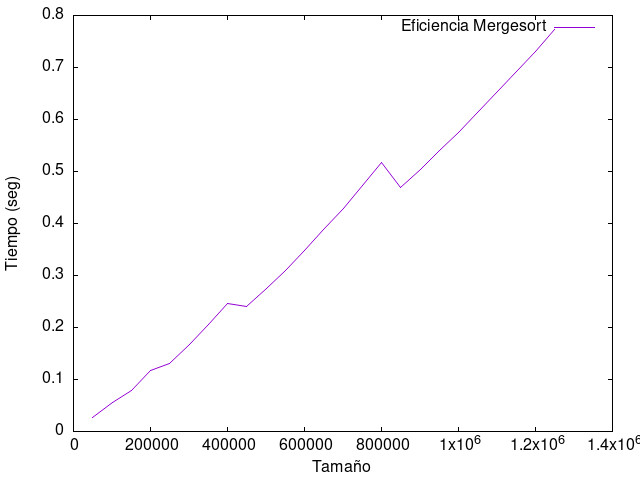
\includegraphics[scale = 0.8]{mergesort.png}
\end{figure}

Al calcular la eficiencia híbrida de Mergesort en gnuplot, obtenemos:
\begin{minted}{text}
Ajustada a la fórmula a0*x*log(x) + a1
iter  	chisq   	delta/lim  lambda   a0
   0 2.6033979525e+15   0.00e+00  1.02e+07	1.000000e+00
   * 9.3808481861e-04   5.78e-11  1.02e+04	1.418029e-08
iter  	chisq   	delta/lim  lambda   a0

After 5 iterations the fit converged.
final sum of squares of residuals : 0.000938085
rel. change during last iteration : -5.77881e-16

degrees of freedom	(FIT_NDF)                       : 24
rms of residuals  	(FIT_STDFIT) = sqrt(WSSR/ndf)   : 0.00625195
variance of residuals (reduced chisquare) = WSSR/ndf   : 3.90869e-05

Final set of parameters        	Asymptotic Standard Error
=======================        	==========================
a0          	= 1.41803e-08  	+/- 1.225e-10	(0.8641%)
a1               = 0.001932       +/- 0.0006271    (32.68%)
\end{minted}

La función ajustada al algoritmo Mergesort para esta ejecución es:

\[\num{1.41803e-08}n\log(n) + 0.001932\]

La gráfica del ajuste queda:
\begin{figure}[H]
  \centering
  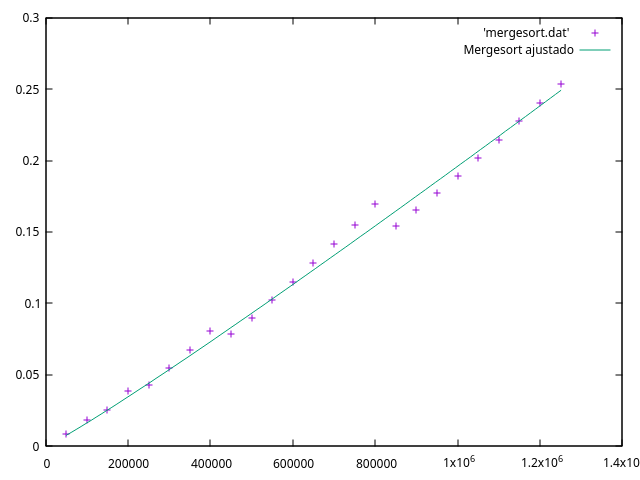
\includegraphics[scale = 1]{AjusteMergesort.png}
  \caption{Ajuste de Mergesort}
\end{figure}


\subsubsection{Ordenación por Quicksort}
Junto a MergeSort, es el algoritmo más rápido de los 8 que hemos visto.

\newpage
La función utilizada es la siguiente:

\begin{minted}{c++}
inline void quicksort(int T[], int num_elem)
static void quicksort_lims(int T[], int inicial, int final)
{
  int k;
  if (final - inicial < UMBRAL_QS) {
    insercion_lims(T, inicial, final);
  } else {
    dividir_qs(T, inicial, final, k);
    quicksort_lims(T, inicial, k);
    quicksort_lims(T, k + 1, final);
  };
}
\end{minted}

Tras compilar y ejecutar \textcolor{ForestGreen}{\textbf{\code{./quicksort}}}:

\begin{longtable}{|c|c|}
\hline
\textbf{Tamaño}  & \textbf{Tiempo(seg)} \\ \hline
50000   & 0.0157172   \\ \hline
100000  & 0.0325483   \\ \hline
150000  & 0.0496276   \\ \hline
200000  & 0.0683057   \\ \hline
250000  & 0.0857514   \\ \hline
300000  & 0.105036    \\ \hline
350000  & 0.123697    \\ \hline
400000  & 0.142723    \\ \hline
450000  & 0.160988    \\ \hline
500000  & 0.178935    \\ \hline
550000  & 0.19783     \\ \hline
600000  & 0.218152    \\ \hline
650000  & 0.237553    \\ \hline
700000  & 0.256666    \\ \hline
750000  & 0.281156    \\ \hline
800000  & 0.296435    \\ \hline
850000  & 0.315857    \\ \hline
900000  & 0.337722    \\ \hline
950000  & 0.360285    \\ \hline
1000000 & 0.376351    \\ \hline
1050000 & 0.398741    \\ \hline
1100000 & 0.417686    \\ \hline
1150000 & 0.4358      \\ \hline
1200000 & 0.455506    \\ \hline
1250000 & 0.473686    \\ \hline
\end{longtable}


Al graficar los datos vemos lo siguiente:

\begin{figure}[H]
  \centering
  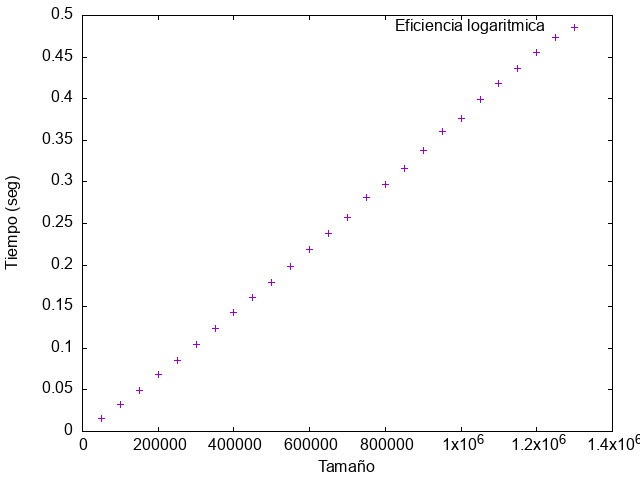
\includegraphics[scale = 0.9]{quicksort.jpeg}
  \caption{Eficiencia Algoritmo QuickSort}
\end{figure}

\newpage

A pesar de parecer lineal, en realidad es logaritmica pues lo vamos a comprobar ahora mismo:
\begin{minted}{text}

FIT:    data read from 'quicksort.dat'
        format = z
        #datapoints = 25
        residuals are weighted equally (unit weight)

function used for fitting: f(x)
	f(x) = a*x*log(x) + b
fitted parameters initialized with current variable values

iter      chisq       delta/lim  lambda   a             b
   0 6.6724879056e-05   0.00e+00  1.96e-01    2.710439e-08   2.021386e-03
   1 6.6724879056e-05   0.00e+00  1.96e+00    2.710439e-08   2.021386e-03

After 1 iterations the fit converged.
final sum of squares of residuals : 6.67249e-05
rel. change during last iteration : 0

Final set of parameters            Asymptotic Standard Error
=======================            ==========================
a               = 2.71044e-08      +/- 6.623e-11    (0.2444%)
b               = 0.00202139       +/- 0.0006759    (33.44%)

correlation matrix of the fit parameters:
                a      b
a               1.000
b              -0.864  1.000
\end{minted}

Quedando la fórmula ajustada como:
 \[ \num{2.71044e-08}\,n\log(n)+0.00202139 \]

La gráfica ajustada resultante es:
\begin{figure}[H]
  \centering
  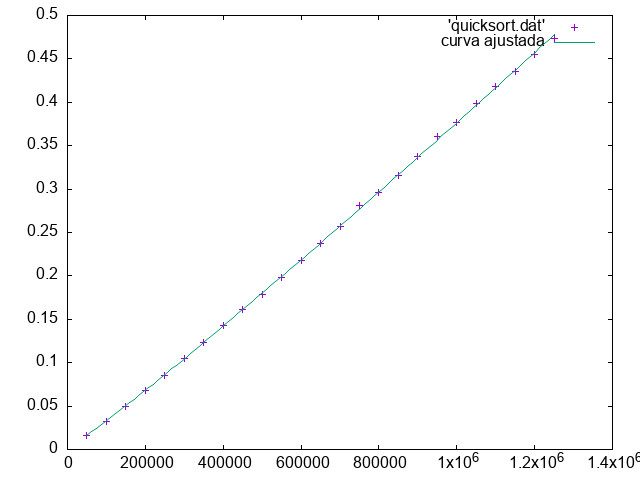
\includegraphics[scale = 0.9]{AjusteQuicksort.jpeg}
  \caption{Ajuste de Quicksort}
\end{figure}

\section{Otros Algoritmos}

\subsection{Eficiencia n³}

\subsubsection{Algoritmo de Floyd}
A continuación, a vemos un algoritmo que tiene la finalidad de calcular el costo del mínimo camino de un grafo dirigido.

Para calcularlo siguiendo las instrucciones del guión hemos ejecutado el algoritmo con la macro del guión, variando su tamaño de 50 a 50 hasta 1250. Mostramos la siguiente tabla con los datos del archivo generado \code{.dat}.

\newpage

El código de Floyd utilizado es:

\begin{minted}{c++}
void Floyd(int **M, int dim)
{
	for (int k = 0; k < dim; k++)
	  for (int i = 0; i < dim;i++)
	    for (int j = 0; j < dim;j++)
	      {
		int sum = M[i][k] + M[k][j];
	    	M[i][j] = (M[i][j] > sum) ? sum : M[i][j];
	      }
}
\end{minted}


La tabla de datos del floyd es:
\begin{longtable}{|c|c|}
\hline
\textbf{Tamaño} & \textbf{Tiempo(seg)} \\ \hline
50     & 0.00189273  \\ \hline
100    & 0.0112866   \\ \hline
150    & 0.0175568   \\ \hline
200    & 0.0525859   \\ \hline
250    & 0.0895145   \\ \hline
300    & 0.191243    \\ \hline
350    & 0.217314    \\ \hline
400    & 0.330062    \\ \hline
450    & 0.517893    \\ \hline
500    & 0.697055    \\ \hline
550    & 0.933725    \\ \hline
600    & 1.27572     \\ \hline
650    & 1.49303     \\ \hline
700    & 2.02039     \\ \hline
750    & 2.46124     \\ \hline
800    & 2.96186     \\ \hline
850    & 3.5521      \\ \hline
900    & 4.10995     \\ \hline
950    & 4.81961     \\ \hline
1000   & 5.70665     \\ \hline
1050   & 6.56104     \\ \hline
1100   & 7.47344     \\ \hline
1150   & 8.87397     \\ \hline
1200   & 9.59515     \\ \hline
1250   & 10.9697     \\ \hline
\end{longtable}


Tras modificar el código fuente y compilar, obtenemos los siguientes datos del \code{.dat}:

\begin{figure}[H]
  \centering
  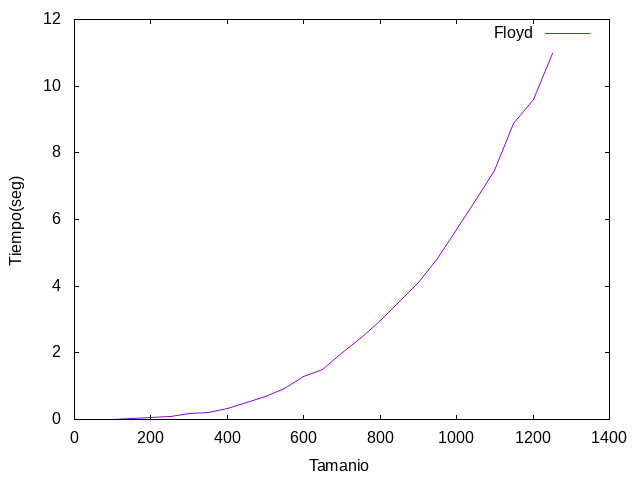
\includegraphics[scale = 1]{floyd.png}
  \caption{Algoritmo Floyd}
\end{figure}

\newpage

El ajuste/búsqueda de variables ocultas genera el siguiente log:

\begin{minted}{text}
************************************************************************
Mon Mar 21 15:30:04 2022


FIT:	data read from "floyd.dat"
    	format = z
    	#datapoints = 25
    	residuals are weighted equally (unit weight)

function used for fitting: f(x)
    f(x) = a0*x*x*x+a1*x*x+a2*x+a3
fitted parameters initialized with current variable values

iter  	chisq   	delta/lim  lambda   a0
   0 1.5636145726e+19   0.00e+00  3.95e+08	1.000000e+00
  12 1.3210841975e-01  -1.85e-02  3.95e-04	5.093144e-09

After 12 iterations the fit converged.
final sum of squares of residuals : 0.132108
rel. change during last iteration : -1.85173e-07

degrees of freedom	(FIT_NDF)                    	: 21
rms of residuals  	(FIT_STDFIT) = sqrt(WSSR/ndf)	: 0.079315
variance of residuals (reduced chisquare) = WSSR/ndf   : 0.00629088

Final set of parameters        	Asymptotic Standard Error
=======================        	==========================
a0          	= 5.09314e-09  	+/- 4.346e-10	(8.534%)
a1          	= 9.66697e-07  	+/- 8.585e-07	(88.81%)
a2          	= -0.000409019 	+/- 0.0004853	(118.6%)
a3          	= 0.0393051    	+/- 0.0743   	(189%)

correlation matrix of the fit parameters:
            	a0     a1      a2      a3
a0          	1.000
a1         	-0.987  1.000
a2          	0.926 -0.973  1.000
a3         	-0.719  0.795 -0.898  1.000
\end{minted}

\newpage

La función resultado del ajuste:

\[f(x)=\num{5.09314e-09}\;x³ + \num{9.66697e-07}\;x² - 0.000409019x + 0.0393051\]

La gráfica ajustada queda:

\begin{figure}[H]
  \centering
  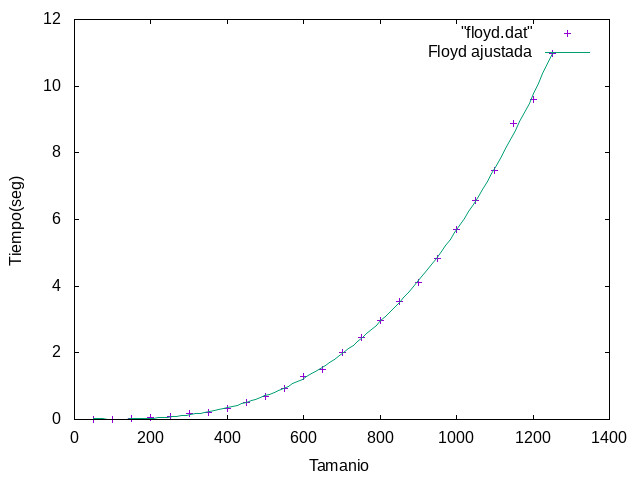
\includegraphics[scale = 0.9]{AjusteFloyd.png}
  \caption{Floyd Ajustado}
\end{figure}

\subsubsection{Algoritmo de dijkstra}
A continuación, vemos el algoritmo recursivo de Dijkstra un algoritmo que tiene el mismo fin pero utiliza un procedimiento recursivo.

\newpage

El código utilizado es el siguiente:

\begin{minted}{c++}
 void Dijkstra(int **M, int **Sal, int dim, int src) // adjacency matrix
{
	int dist[dim]; // integer array to calculate minimum distance
	bool Tset[dim];// boolean array to mark visted/unvisted

	// set the nodes with infinity distance
	for(int i = 0; i<dim; i++)
	{
		dist[i] = INT_MAX;
		Tset[i] = false;
	}

	dist[src] = 0;   // Source vertex distance is set to zero.

	for(int k = 0; k<dim; k++)
	{
		int m=minimumDist(dist,Tset,dim);
		Tset[m]=true;// m with minimum distance included in Tset.
		for(int i = 0; i<dim; i++)
		{
			// Updating the minimum distance
			if(!Tset[i] && dist[m]!=INT_MAX
              && dist[m]+M[m][i]<dist[i])
				dist[i]=dist[m]+M[m][i];
		}
	}
	for(int i = 0; i<dim; i++)
	   Sal[src][i]=dist[i];
}
\end{minted}

La tabla de datos de dijkstra:

\begin{longtable}{|l|l|}
\hline
\textbf{Tamaño} & \textbf{Tiempo(seg)} \\ \hline
50     & 0.00283111  \\ \hline
100    & 0.00949102  \\ \hline
150    & 0.0285824   \\ \hline
200    & 0.0704248   \\ \hline
250    & 0.136364    \\ \hline
300    & 0.171888    \\ \hline
350    & 0.259129    \\ \hline
400    & 0.369816    \\ \hline
450    & 0.515604    \\ \hline
500    & 0.690241    \\ \hline
550    & 0.822436    \\ \hline
600    & 0.962625    \\ \hline
650    & 1.34316     \\ \hline
700    & 1.52782     \\ \hline
750    & 2.07249     \\ \hline
800    & 2.50367     \\ \hline
850    & 2.90906     \\ \hline
900    & 3.4613      \\ \hline
950    & 4.30861     \\ \hline
1000   & 5.00108     \\ \hline
1050   & 5.57536     \\ \hline
1100   & 6.00137     \\ \hline
1150   & 6.79705     \\ \hline
1200   & 8.28284     \\ \hline
1250   & 9.33255     \\ \hline
\end{longtable}


Cuya gráfica asociada es:
\begin{figure}[H]
  \centering
  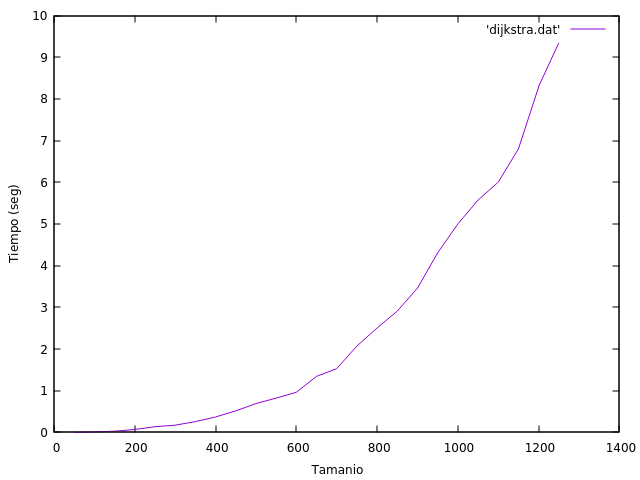
\includegraphics[scale = 0.7]{dijkstra.png}
\end{figure}

Calculamos el ajuste con gnuplot:
\begin{minted}{text}
*************************************************************************
Mon Mar 21 15:20:52 2022


FIT:    data read from 'dijkstra.dat'
        format = z
        #datapoints = 25
        residuals are weighted equally (unit weight)

function used for fitting: f(x)
	f(x)=a3*x*x*x+a2*x*x+a1*x+a0
fitted parameters initialized with current variable values

iter      chisq       delta/lim  lambda       a3             a2
   0 1.5636145755e+19   0.00e+00  3.95e+08    1.000000e+00   1.000000e+00
  12 4.3580634335e-01  -6.12e-03  3.95e-04    4.705614e-09  -1.473596e-07

After 12 iterations the fit converged.
final sum of squares of residuals : 0.435806
rel. change during last iteration : -6.11875e-08

degrees of freedom    (FIT_NDF)                        : 21
rms of residuals      (FIT_STDFIT) = sqrt(WSSR/ndf)    : 0.144058
variance of residuals (reduced chisquare) = WSSR/ndf   : 0.0207527

Final set of parameters            Asymptotic Standard Error
=======================            ==========================
a3              = 4.70561e-09      +/- 7.894e-10    (16.78%)
a2              = -1.4736e-07      +/- 1.559e-06    (1058%)
a1              = 0.000192697      +/- 0.0008814    (457.4%)
a0              = -0.00275768      +/- 0.135        (4894%)

correlation matrix of the fit parameters:
                a3     a2     a1     a0
a3              1.000
a2             -0.987  1.000
a1              0.926 -0.973  1.000
a0             -0.719  0.795 -0.898  1.000
\end{minted}

\newpage

La formula ajustada es:
\[f(x)= \num{4.70561e-09}x³ - \num{1.4736e-07}x² + 0.000192697x - 0.00275768\]

La gráfica con el ajuste queda:
\begin{figure}[H]
  \centering
  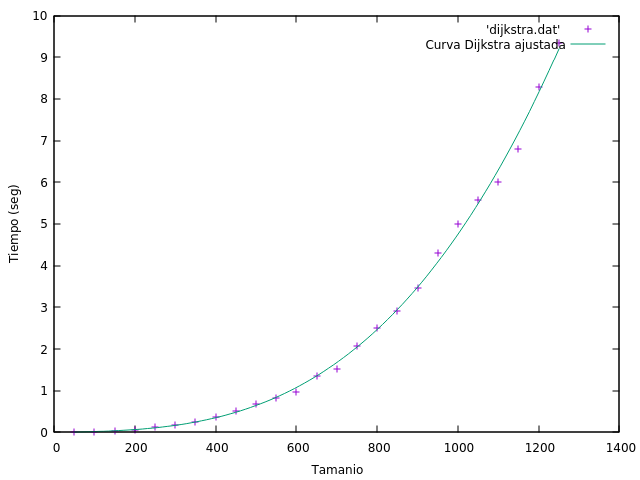
\includegraphics[scale = 0.7]{AjusteDijkstra.png}
\end{figure}

A continuación, vamos a probar otros ajustes que no son buenos para el algoritmo de Dijkstra. Probamos un ajuste lineal.

\begin{figure}[H]
  \centering
  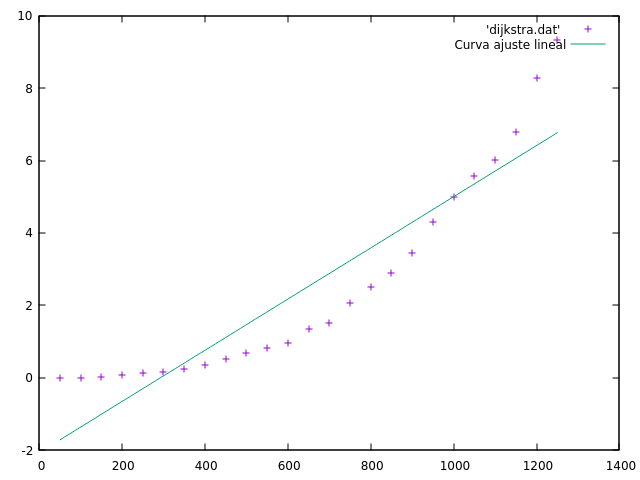
\includegraphics[scale = 0.7]{AjusteLinealDijkstra.png}
\end{figure}

Como podemos observar el ajuste es completamente malo, no es para nada la función real. Probamos con un ajuste con n⁴:

\begin{figure}[H]
  \centering
  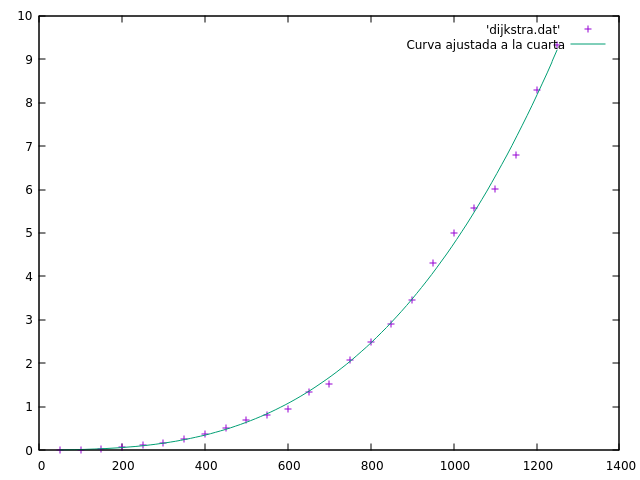
\includegraphics[scale = 0.7]{AjusteCuartaDijkstra.png}
  \caption{Ajuste n⁴ de Dijkstra}
\end{figure}

Podemos observar que en ciertos tamaños pequeños del algoritmo de Dijkstra, con un ajuste superior al suyo propio, el ajuste queda bien.

\subsection{Eficiencia aⁿ}
Los algoritmos de orden aⁿ son el algoritmo de hanoi y el algoritmo recursivo de fibonacci que se utilizan respectivamente para resolver el famoso problema de las torres de Hanoi y calcular los números de la sucesión de Fibonacci.

\subsubsection{Algoritmo de fibonacci}

El algoritmo de fibonacci es un clásico de la programación y de las matemáticas. Su código recursivo es bastante simple:

\begin{minted}{c++}
int fibo(int n)
{
  if (n < 2)
    return 1;
  else
    return fibo(n-1) + fibo(n-2);
}
\end{minted}

Con unos datos suficientemente altos podemos obtener su eficiencia, obteniendo la tabla:

\begin{longtable}{|c|c|}
\hline
\textbf{Tamaño} & \textbf{Tiempo(seg)} \\ \hline
2      & 3.5e-07     \\ \hline
4      & 3.9e-07     \\ \hline
6      & 7.31e-07    \\ \hline
8      & 1,34E-03    \\ \hline
10     & 2,58E-03    \\ \hline
12     & 5,01E-03    \\ \hline
14     & 1.0349e-05  \\ \hline
16     & 2.4075e-05  \\ \hline
18     & 5.6516e-05  \\ \hline
20     & 0.000141576 \\ \hline
22     & 0.000362882 \\ \hline
24     & 0.000991363 \\ \hline
26     & 0.00248774  \\ \hline
28     & 0.00645781  \\ \hline
30     & 0.0172408   \\ \hline
32     & 0.045158    \\ \hline
34     & 0.11677     \\ \hline
36     & 0.304076    \\ \hline
38     & 0.799934    \\ \hline
40     & 2.08225     \\ \hline
42     & 5.75886     \\ \hline
44     & 14.5311     \\ \hline
46     & 37.9627     \\ \hline
48     & 98.5858     \\ \hline
50     & 258313      \\ \hline
\end{longtable}


\newpage

La gráfica queda:
\begin{figure}[H]
  \centering
  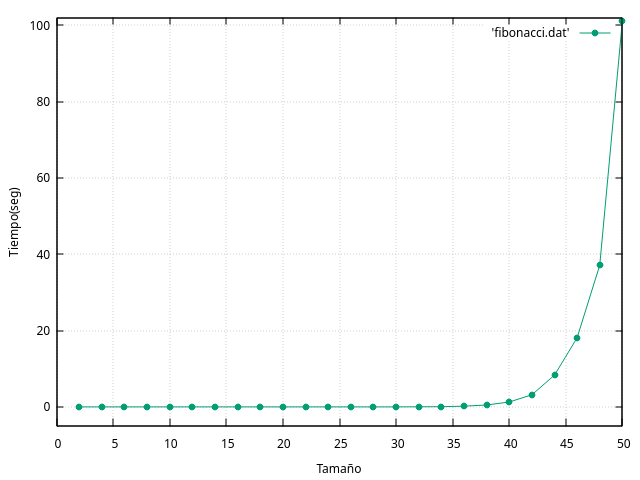
\includegraphics[scale = 1]{fibonacci.png}
  \caption{Algoritmo de Fibonacci}
\end{figure}

\newpage

El ajuste del algoritmo en gnuplot es el siguiente:

\begin{minted}{text}

*************************************************************************
Sun Mar 20 21:44:24 2022


FIT:    data read from 'fibonacci.dat'
        format = z
        #datapoints = 25
        residuals are weighted equally (unit weight)

function used for fitting: f(x)
	f(x) = a*1.618**x + b
fitted parameters initialized with current variable values

iter      chisq       delta/lim  lambda   a             b
   0 9.2543992530e+20   0.00e+00  4.30e+09    1.000000e+00   1.000000e+00
   5 2.1871058673e+01  -2.44e-05  4.30e+04    9.139440e-09   1.000000e+00

After 5 iterations the fit converged.
final sum of squares of residuals : 21.8711
rel. change during last iteration : -2.44244e-10

degrees of freedom    (FIT_NDF)                        : 23
rms of residuals      (FIT_STDFIT) = sqrt(WSSR/ndf)    : 0.975149
variance of residuals (reduced chisquare) = WSSR/ndf   : 0.950916

Final set of parameters            Asymptotic Standard Error
=======================            ==========================
a               = 9.13944e-09      +/- 3.359e-11    (0.3676%)
b               = 1                +/- 0.2044       (20.44%)

correlation matrix of the fit parameters:
                a      b
a               1.000
b              -0.299  1.000
\end{minted}

La función ajuste obtenida:

\[f(x)=\num{9.13944e-09}\left(\frac{1+\sqrt{5}}{2}\right)^n + 1\]

\newpage

La gráfica ajustada es:

\begin{figure}[H]
  \centering
  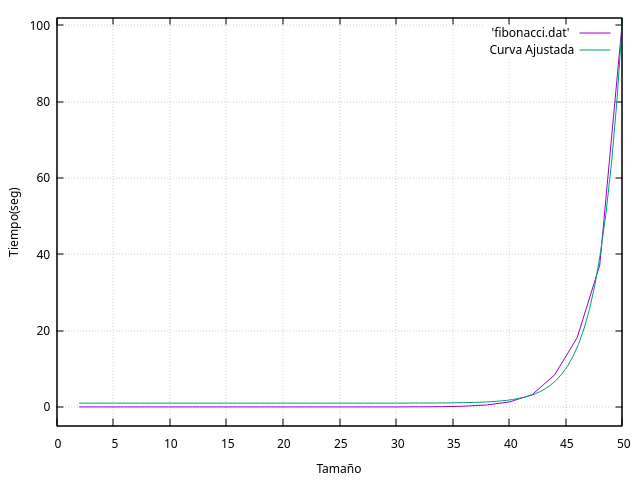
\includegraphics[scale = 0.9]{AjusteFibonacci.png}
  \caption{Ajuste de Fibonacci}
\end{figure}

\subsubsection{Algoritmo de hanoi}

El código utilizado para el algoritmo de hanoi es:
\begin{minted}{c++}
void hanoi (int M, int i, int j)
{
  if (M > 0)
	{
  	hanoi(M-1, i, 6-i-j);
  	cout << i << " -> " << j << endl;
  	hanoi (M-1, 6-i-j, j);
  }
}
\end{minted}

\newpage

La tabla de datos resultante de este algoritmo es la siguiente:

\begin{longtable}{|c|c|}
\hline
\textbf{Tamaño}                   & \textbf{Tiempo(seg)} \\ \hline
3                        & 3.81e-07    \\ \hline
4                        & 2.4e-07     \\ \hline
5                        & 3.4e-07     \\ \hline
6                        & 4.91e-07    \\ \hline
7                        & 8.12e-07    \\ \hline
8                        & 1.392e-06   \\ \hline
9                        & 5.701e-06   \\ \hline
10                       & 4.85e-06    \\ \hline
11                       & 9.338e-06   \\ \hline
12                       & 1.8375e-05  \\ \hline
13                       & 3.631e-05   \\ \hline
14                       & 7.5824e-05  \\ \hline
15                       & 0.000144055 \\ \hline
16                       & 0.000289803 \\ \hline
17                       & 0.000578454 \\ \hline
18                       & 0.00115254  \\ \hline
19                       & 0.00230918  \\ \hline
20                       & 0.00461556  \\ \hline
21                       & 0.00921158  \\ \hline
22                       & 0.0184436   \\ \hline
23                       & 0.0367877   \\ \hline
24                       & 0.0738795   \\ \hline
25                       & 0.147934    \\ \hline
26                       & 0.295861    \\ \hline
27                       & 0.592275    \\ \hline
28                       & 1.18338     \\ \hline
29                       & 2.36899     \\ \hline
30                       & 4.7301      \\ \hline
31                       & 9.49097     \\ \hline
32                       & 18.998      \\ \hline
33                       & 37.9925     \\ \hline
\end{longtable}


\newpage

Quedando la siguiente gráfica:

\begin{figure}[H]
  \centering
  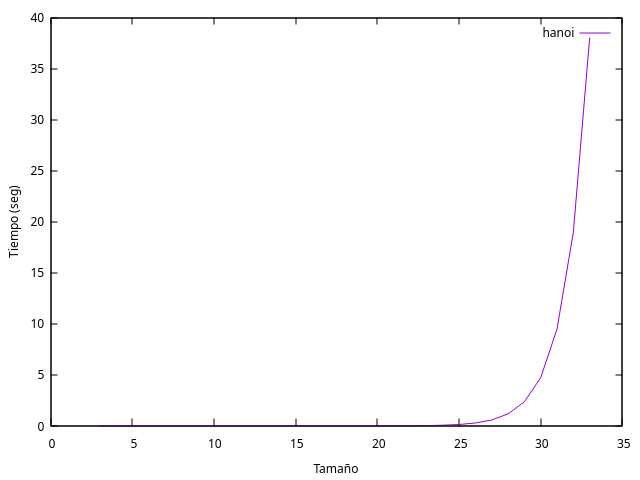
\includegraphics[scale = 0.7]{hanoi.png}
  \caption{Algoritmo de hanoi}
\end{figure}

El ajuste y búsqueda de constantes ocultas en gnuplot queda:

\begin{minted}{text}
Ajustada a la fórmula a0*2x
iter  	chisq   	delta/lim  lambda   a0
   0 9.3672982738e+03   0.00e+00  2.53e+01	1.418029e-08
   4 4.5210289275e-04  -2.18e-09  2.53e-03	4.422579e-09
iter  	chisq   	delta/lim  lambda   a0

After 4 iterations the fit converged.
final sum of squares of residuals : 0.000452103
rel. change during last iteration : -2.1823e-14

degrees of freedom	(FIT_NDF)                    	: 30
rms of residuals  	(FIT_STDFIT) = sqrt(WSSR/ndf)	: 0.00388202
variance of residuals (reduced chisquare) = WSSR/ndf   : 1.50701e-05

Final set of parameters        	Asymptotic Standard Error
=======================        	==========================
a0          	= 4.42258e-09  	+/- 3.914e-13	(0.00885%)
\end{minted}

\newpage
La función ajustada que se obtiene es la siguiente:

\[ f(x)= \num{4.42258e-09} \times 2^x \]


La gráfica resultante del ajuste es:

\begin{figure}[H]
  \centering
  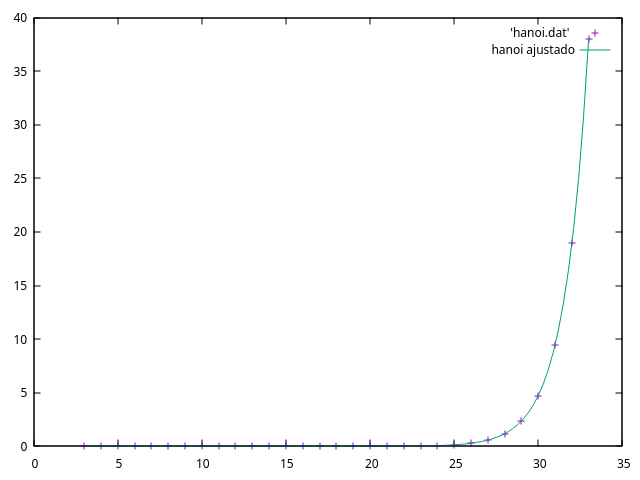
\includegraphics[scale = 0.9]{AjusteHanoi.png}
  \caption{Ajuste Hanoi}
\end{figure}


\section{Variación de la eficiencia empírica por factores externos}
Hemos elegido el algoritmo de burbuja para ver como se comporta con diferentes grados de optimización, distintos SO e incluso modos de rendimiento en el mismo ordenador.

\subsection{Flags de Optimización}
\begin{table}
\parbox{.45\linewidth}{
\centering
\begin{tabular}{|c|c|}
\hline
\textbf{Tamaño} & \textbf{Tiempo(seg)} \\ \hline
5000   & 0.0593889   \\ \hline
10000  & 0.214639    \\ \hline
15000  & 0.497034    \\ \hline
20000  & 0.920987    \\ \hline
25000  & 1.43304     \\ \hline
30000  & 2.09295     \\ \hline
35000  & 2.86473     \\ \hline
40000  & 3.77359     \\ \hline
45000  & 4.80492     \\ \hline
50000  & 5.90436     \\ \hline
55000  & 7.18508     \\ \hline
60000  & 8.52722     \\ \hline
65000  & 10.0494     \\ \hline
70000  & 11.6697     \\ \hline
75000  & 13.4947     \\ \hline
80000  & 15.3079     \\ \hline
85000  & 17.3202     \\ \hline
90000  & 19.3166     \\ \hline
95000  & 21.4845     \\ \hline
100000 & 24.2024     \\ \hline
105000 & 26.3043     \\ \hline
110000 & 28.9074     \\ \hline
115000 & 31.5045     \\ \hline
120000 & 34.3248     \\ \hline
125000 & 37.2732     \\ \hline
\end{tabular}

\caption{-Ofast}
}
\hfill
\parbox{.45\linewidth}{
\centering
\begin{tabular}{|c|c|}
\hline
\textbf{Tamaño} & \textbf{Tiempo(seg)} \\ \hline
5000   & 0.0353615   \\ \hline
10000  & 0.12893     \\ \hline
15000  & 0.279444    \\ \hline
20000  & 0.519757    \\ \hline
25000  & 0.848564    \\ \hline
30000  & 1.22494     \\ \hline
35000  & 1.69467     \\ \hline
40000  & 2.22243     \\ \hline
45000  & 2.86132     \\ \hline
50000  & 3.54748     \\ \hline
55000  & 4.28462     \\ \hline
60000  & 5.1476      \\ \hline
65000  & 6.03558     \\ \hline
70000  & 7.023       \\ \hline
75000  & 8.09728     \\ \hline
80000  & 9.21789     \\ \hline
85000  & 10.6009     \\ \hline
90000  & 11.7605     \\ \hline
95000  & 13.1332     \\ \hline
100000 & 14.4467     \\ \hline
105000 & 16.195      \\ \hline
110000 & 17.6103     \\ \hline
115000 & 19.6109     \\ \hline
120000 & 21.3958     \\ \hline
125000 & 37.8755     \\ \hline
\end{tabular}

\caption{-Os}
}
\end{table}

\newpage

\begin{table}[H]
\parbox{.3\linewidth}{
\centering
\begin{longtable}{|c|c|}
\hline
\textbf{Tamaño} & \textbf{Tiempo(seg)} \\ \hline
5000   & 0.040981    \\ \hline
10000  & 0.121329    \\ \hline
15000  & 0.263826    \\ \hline
20000  & 0.514343    \\ \hline
25000  & 0.794101    \\ \hline
30000  & 1.17507     \\ \hline
35000  & 1.61848     \\ \hline
40000  & 2.21165     \\ \hline
45000  & 2.89982     \\ \hline
50000  & 3.46264     \\ \hline
55000  & 4.26109     \\ \hline
60000  & 5.10696     \\ \hline
65000  & 6.01018     \\ \hline
70000  & 7.32373     \\ \hline
75000  & 8.25187     \\ \hline
80000  & 9.10546     \\ \hline
85000  & 10.8578     \\ \hline
90000  & 11.9108     \\ \hline
95000  & 13.0263     \\ \hline
100000 & 14.8928     \\ \hline
105000 & 15.9502     \\ \hline
110000 & 17.4961     \\ \hline
115000 & 19.4555     \\ \hline
120000 & 21.0152     \\ \hline
125000 & 22.5864     \\ \hline
\end{longtable}

\caption{-O1}
}
\quad
\parbox{.3\linewidth}{
\centering
\begin{longtable}{|c|c|}
\hline
\textbf{Tamaño} & \textbf{Tiempo(seg)} \\ \hline
5000   & 0.0379419   \\ \hline
10000  & 0.147648    \\ \hline
15000  & 0.306699    \\ \hline
20000  & 0.586954    \\ \hline
25000  & 0.89294     \\ \hline
30000  & 1.3054      \\ \hline
35000  & 1.78492     \\ \hline
40000  & 2.37671     \\ \hline
45000  & 3.03008     \\ \hline
50000  & 4.10658     \\ \hline
55000  & 4.5193      \\ \hline
60000  & 5.4013      \\ \hline
65000  & 6.37231     \\ \hline
70000  & 7.44308     \\ \hline
75000  & 8.46187     \\ \hline
80000  & 9.67369     \\ \hline
85000  & 10.9855     \\ \hline
90000  & 12.2241     \\ \hline
95000  & 13.6452     \\ \hline
100000 & 15.2075     \\ \hline
105000 & 16.7299     \\ \hline
110000 & 18.9098     \\ \hline
115000 & 21.1148     \\ \hline
120000 & 22.4663     \\ \hline
125000 & 24.0422     \\ \hline
\end{longtable}

\caption{-O2}
}
\quad
\parbox{.3\linewidth}{
\centering
\begin{longtable}{|c|c|}
\hline
\textbf{Tamaño} & \textbf{Tiempo(seg)} \\ \hline
5000   & 0.0810466   \\ \hline
10000  & 0.22743     \\ \hline
15000  & 0.515814    \\ \hline
20000  & 0.909461    \\ \hline
25000  & 1.43552     \\ \hline
30000  & 2.11438     \\ \hline
35000  & 2.88025     \\ \hline
40000  & 3.76616     \\ \hline
45000  & 4.825       \\ \hline
50000  & 5.90919     \\ \hline
55000  & 7.17914     \\ \hline
60000  & 8.53562     \\ \hline
65000  & 10.0452     \\ \hline
70000  & 11.6576     \\ \hline
75000  & 13.3829     \\ \hline
80000  & 15.2273     \\ \hline
85000  & 17.7326     \\ \hline
90000  & 19.4547     \\ \hline
95000  & 21.5236     \\ \hline
100000 & 23.8546     \\ \hline
105000 & 26.5079     \\ \hline
110000 & 28.8266     \\ \hline
115000 & 31.6179     \\ \hline
120000 & 35.3284     \\ \hline
125000 & 37.725      \\ \hline
\end{longtable}

\caption{-O3}
}
\end{table}

\newpage

La grafica comparativa resultante es:
\begin{figure}[H]
  \centering
  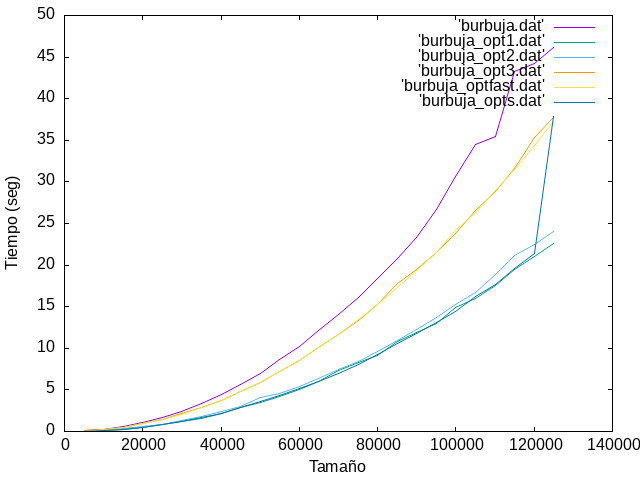
\includegraphics[scale = 0.7]{allBurbujas.png}
\end{figure}

\subsection{Distintos Sistemas Operativos}
Además hemos probado el algoritmo de Burbuja en distinos Sistemas operativos como Windows 10 y MacOS:

\begin{figure}[H]
  \centering
  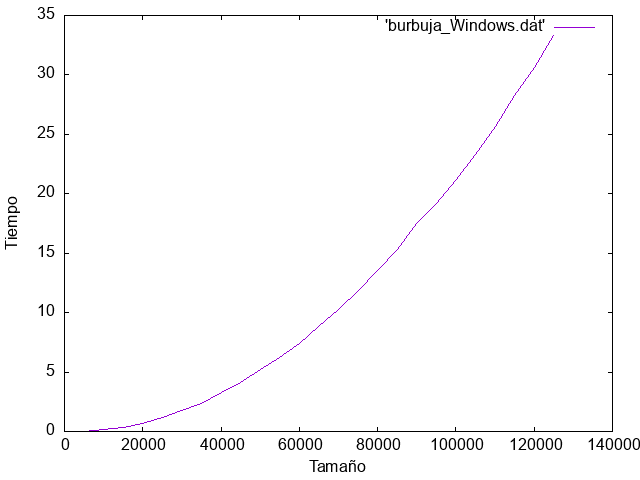
\includegraphics[scale = 0.7]{burbujaWindows.png}
\end{figure}

\begin{figure}[H]
  \centering
  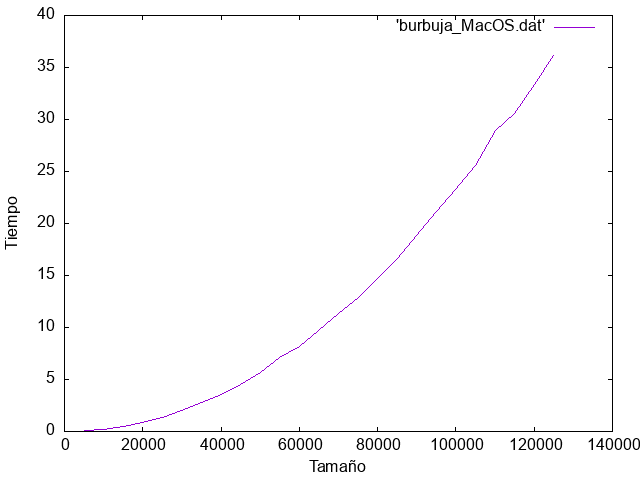
\includegraphics[scale = 0.7]{burbujaMacOS.png}
\end{figure}

Tras la comparativa final, sorprendentemente en windows tarda menos:
\begin{figure}[H]
  \centering
  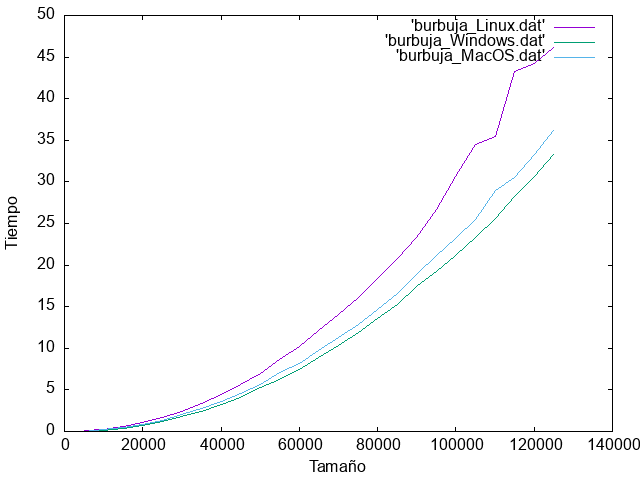
\includegraphics[scale = 0.8]{burbujaOS.png}
  \caption{Comparación entre SO}
\end{figure}

\section{Los tiempos de todos los algoritmos}
En esta sección compararemos todos los algoritmos en la misma gráfica y veremos la diferencia de eficiencia entre los distintos órdenes de algoritmos que hemos medido.


\begin{figure}[H]
  \centering
  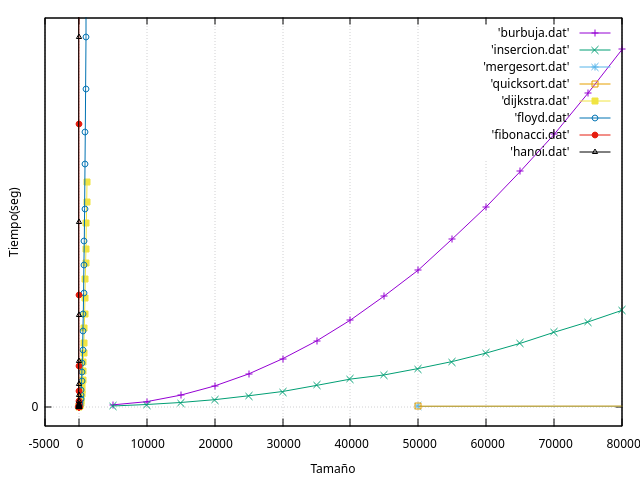
\includegraphics[scale = 1]{TodosAlgoritmos.png}
  \caption{La eficiencia de todos los algoritmos}
\end{figure}


Ahora obtendremos específicamente podemos ver la diferencia en la gráfica de los algoritmos de ordenación.

\begin{figure}[H]
  \centering
  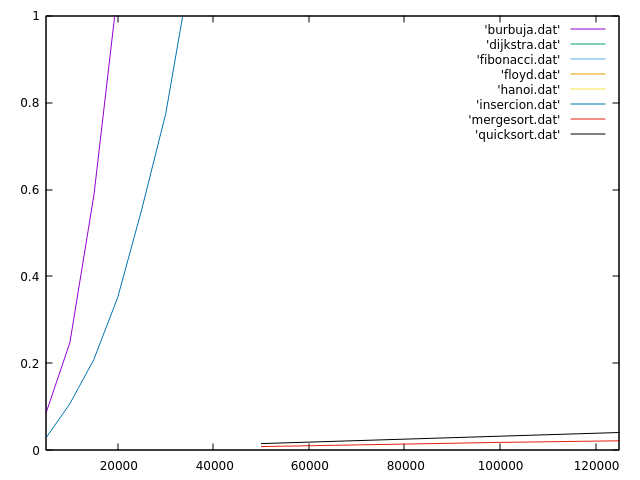
\includegraphics[scale = 0.7]{AlgoritmosOrdenacion.png}
  \caption{La eficiencia de los algorítmos de ordenación}
\end{figure}

Las gráficas por eficiencia de algoritmos son:

\begin{itemize}
 \item Eficiencia n²:
  \begin{figure}[H]
    \centering
    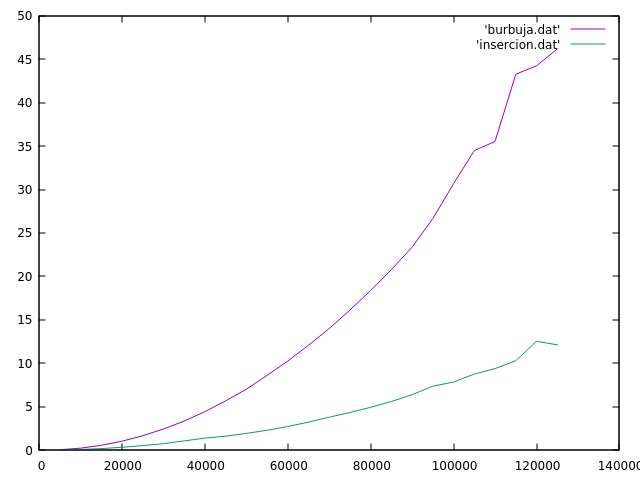
\includegraphics[scale = 0.5]{BurbujaInsercion.png}
    \caption{La eficiencia de los algorítmos n²}
  \end{figure}

 \item Eficiencia nlog(n)
   \begin{figure}[H]
    \centering
    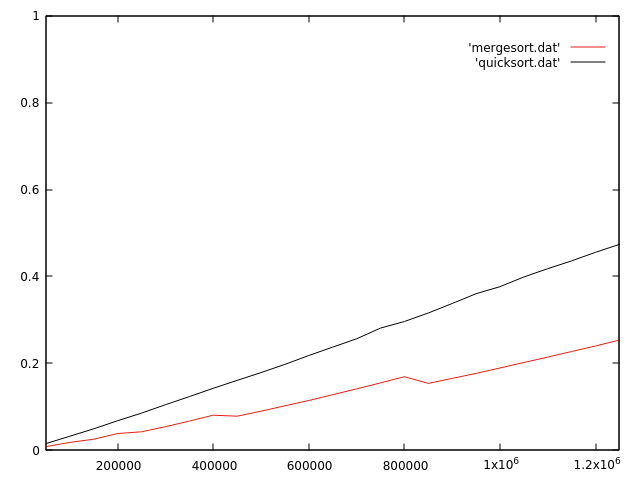
\includegraphics[scale = 0.7]{QuicksortMergesort.png}
  \end{figure}

  \item Eficiencia n³
    \begin{figure}[H]
    \centering
    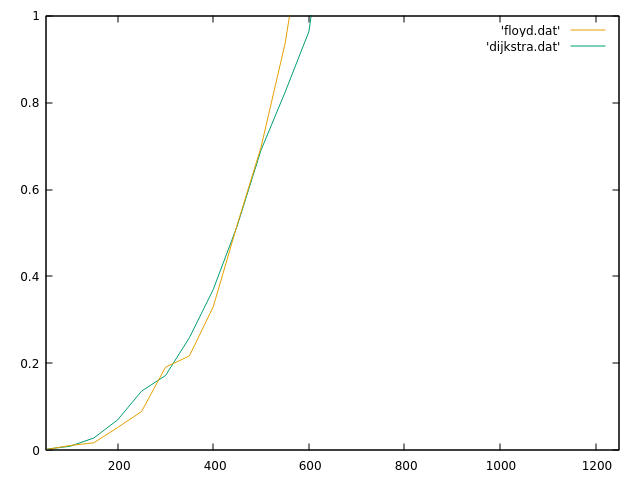
\includegraphics[scale = 0.7]{FloydDijkstra.png}
    \caption{La eficiencia de los algorítmos n³}
  \end{figure}

  \item Eficiencia aⁿ
    \begin{figure}[H]
    \centering
    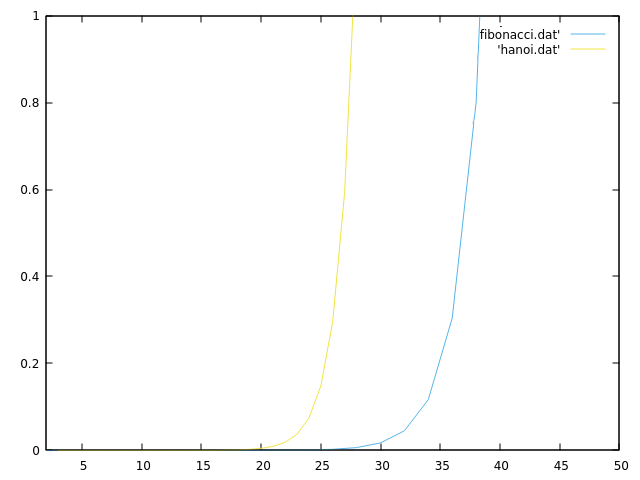
\includegraphics[scale = 0.7]{FibonacciHanoi.png}
    \caption{La eficiencia de los algorítmos aⁿ}
  \end{figure}

\end{itemize}

\vspace{5cm}
 \bibliographystyle{plain}
 \bibliography{biblist}


\end{document}
